\documentclass[a4paper,12pt]{article}
\usepackage{hyperref}
% Required packages
\usepackage[utf8]{inputenc} % UTF-8 character encoding
\usepackage[english]{babel} % Support for English
\usepackage{graphicx} % Insert images
\usepackage{fancyhdr} % Custom headers and footers
\usepackage{tocbibind} % Include bibliography in the table of contents
\usepackage{hyperref}
\usepackage{mathtools}  
\usepackage{setspace} % Control line spacing
\usepackage{enumitem} % Custom lists
\usepackage{titlesec} % Format titles
\usepackage{geometry} % Configure margins
\usepackage{newtxtext,newtxmath} % Times New Roman font
\usepackage{ragged2e} % Justified alignment
\usepackage{url} % Display URLs
\usepackage{array} % Improve tables
\usepackage{pgfgantt} % Gantt charts
\usepackage{lscape} % Landscape mode pages
\usepackage{xcolor} % Custom colors
\usepackage{verbatim} % Verbatim environment
\usepackage{listings} % Display source code

% Configuración de márgenes
\geometry{
	a4paper,
	left=3.5cm,
	right=2.5cm,
	top=2.5cm,
	bottom=2.5cm
}

% Line spacing
\onehalfspacing

% Section title formatting
\titleformat{\section}
{\normalfont\bfseries\large} % Section format: normal, bold, 14pt (LARGE)
{\thesection}{1em}{\MakeUppercase} % Uppercase
\titlespacing*{\section}{0pt}{6pt}{18pt} % Section spacing: 6pt before, 18pt after
\newcommand{\sectionbreak}{\clearpage} % New page for each section

% Subsection title formatting
\titleformat{\subsection}
{\normalfont\bfseries\normalsize} % Subsection format: normal, bold, 12pt (Large)
{\thesubsection}{1em}{}
\titlespacing*{\subsection}{0pt}{6pt}{18pt} % Subsection spacing: 6pt before, 18pt after

% Subsubsection title formatting
\titleformat{\subsubsection}
{\normalfont\bfseries\normalsize} % Subsubsection format: normal, bold, 10pt (large)
{\thesubsubsection}{1em}{}
\titlespacing*{\subsubsection}{0pt}{6pt}{18pt} % Subsubsection spacing: 6pt before, 18pt after

% Formatting for Abstract and Summary
\titleformat{name=\section,numberless}[block]
{\normalfont\bfseries\normalsize\centering}
{}
{0pt}
{}

% Capitalize titles
\addto\captionsenglish{
	\renewcommand{\contentsname}{Table of Contents}
	\renewcommand{\listfigurename}{List of Figures}
	\renewcommand{\listtablename}{List of Tables}
	\renewcommand{\tablename}{Table}
	\renewcommand{\refname}{References}
}

% Header and footer configuration
\pagestyle{fancy}
\fancyhf{}
\fancyhead{} % Remove header content
\fancyfoot[R]{\thepage} % Page number on the bottom right
\renewcommand{\headrulewidth}{0pt} % Remove horizontal line in header
\renewcommand{\footrulewidth}{0pt} % Remove horizontal line in footer

% Redefine Roman numeral page numbering for preliminary pages
\fancypagestyle{plain}{
	\fancyhf{}
	\fancyfoot[R]{\thepage}
	\renewcommand{\thepage}{\roman{page}}
}


\begin{document}
	
	% Include cover page
	\begin{titlepage}
	
	\begin{center}
		
\includegraphics[width=0.6\linewidth]{img/izügenislogo.jpg} 
		\vspace{7pt}
		
		{\fontsize{16}{19.2}\selectfont{\textbf{Istanbul Sabahattin Zaim University}\\}}
		{\fontsize{16}{19.2}\selectfont{\textbf{Faculty of Engineering and Natural Sciences}}\\}
		{\fontsize{16}{19.2}\selectfont{\textbf{Electrical \& Electronics Engineering}}\\}
        {\fontsize{16}{19.2}\selectfont{\textbf{Spring 2024-2025}}\\}

        
		\vspace{1cm}
		{\fontsize{16}{19.2}\selectfont{\textbf{Microcontrollers Lab}\\}}
		\vspace{1cm}
		{\fontsize{16}{19.2}\selectfont{\textbf{Experiment 0}\\}}
		\vspace{1cm}
		{\fontsize{15}{18}\selectfont
			\textbf{Report Template\\}
		}

		\vspace{1cm}
		{\fontsize{16}{19.2}\selectfont\textbf{Prepared By:}\\
			Student Name \\03102xxxx}

		\vspace{1cm}
		{\fontsize{16}{19.2}\selectfont\textbf{Advisors:}\\
			Assist. Prof. Dr. Mohammed JOUDA \\Res. Assist. Furkan Ahmet TAMYİĞİT\\}


        
		\vfill
		
		{\fontsize{16}{19.2}\selectfont{\large\ Month Day, Year \\}}

		
	\end{center}
	
\end{titlepage}
	
	% Use Roman numerals for preliminary pages
	\clearpage
	\pagenumbering{roman}    
	\setcounter{page}{2} % Start at ii
	\renewcommand{\thepage}{\roman{page}}
	
	% Approval Page (commented)
	%\pagestyle{plain}
	%\begin{center}
	\textbf{APPROVAL SHEET}

	\vspace{0.5cm}
	\textbf{Title of the Final Degree Project Proposal}
\end{center}

\vspace{2cm}
Approved by:
\vspace{1cm}

\begin{enumerate}
	\item Signature of the TFG Course Professor: \underline{\hspace{6cm}} \\
	
	\begin{description}
		\item Printed Name: \underline{\hspace{7cm}} \\
		\item Date of approval:
		% You may uncomment the example date below for use,
		% and comment out the underline section if needed.
		%26/07/2020 
		\underline{\hspace{1cm}}/\underline{\hspace{1cm}}/\underline{\hspace{2cm}}
	\end{description}
	
	\vspace{1cm}
	
	\item Signature of the Head of the Research Department: \underline{\hspace{3.5cm}} \\
	
	\begin{description}
		\item Printed Name: \underline{\hspace{7cm}} \\
		\item Date of approval:
		% You may uncomment the example date below for use,
		% and comment out the underline section if needed.
		%26/07/2020 
		\underline{\hspace{1cm}}/\underline{\hspace{1cm}}/\underline{\hspace{2cm}}
	\end{description}
	
\end{enumerate}

	%\thispagestyle{plain} % Ensure page number appears
	
	\newpage
	
	% Compliance Declaration (commented)
	%\pagestyle{plain}
	%\centering\textbf{STATEMENT OF CONFORMITY BY THE ACADEMIC ADVISOR}

\vspace{1cm}
\begin{flushright}
	\textit{City}, \textit{Date}
\end{flushright}
\vspace{1cm}

\begin{flushleft}
	\hspace{1cm} I, \textit{name of the Academic Advisor}, identification number: \textit{ID number}, professor of the Bachelor's Degree Program in Systems Analysis, at the campus/branch \textit{Name of the campus/branch}, hereby express my agreement to supervise the execution of the Final Degree Project titled ``\textit{title of the project}'', by the student \textit{name of the student}, identification number: \textit{ID number}, until its completion within the regulatory timeframe.
\end{flushleft}
\vspace{2cm}

\begin{center}
	\textit{Signature of the academic advisor} \\
	\vspace{0.5cm}
	\underline{\hspace{7cm}} \\
	\textit{Name of the academic advisor}
\end{center}
\vspace{1cm}

	%\thispagestyle{plain} % Ensure page number appears
	
	% Table of Contents (excluded from TOC itself)
	\addtocontents{toc}{\protect\setcounter{tocdepth}{-1}}
	\tableofcontents
	\addtocontents{toc}{\protect\setcounter{tocdepth}{2}}
	\newpage
	
	% List of Tables (excluded from TOC itself)
	\addtocontents{toc}{\protect\setcounter{tocdepth}{-1}}
	\listoftables
	\addtocontents{toc}{\protect\setcounter{tocdepth}{2}}
	\newpage
	
	% List of Figures (excluded from TOC itself)
	\addtocontents{toc}{\protect\setcounter{tocdepth}{-1}}
	\listoffigures
	\addtocontents{toc}{\protect\setcounter{tocdepth}{2}}
	\newpage
	
	% Abstract or Summary
	\pagestyle{plain}
	\begin{minipage}{\textwidth}


	
	\section*{Abstract}
	\addcontentsline{toc}{section}{Abstract}
	\justifying
	\noindent
A long abstract can be written here.\\

\textbf{Keywords:} Keyword1, Keyword2, Keyword3.


\section*{Objectives}
\addcontentsline{toc}{section}{Objectives}
With this experiment we aim to:
\justifying
\noindent
\begin{itemize}
    \item objective1.
    \item objective1.
    \item objective1r.
    \item objective1.
\end{itemize}


\end{minipage}
	\thispagestyle{plain}
	\newpage
	
	% Switch to Arabic numerals
	\pagenumbering{arabic}
	\fancyfoot[R]{\thepage} % Page number on bottom right
	
	% Justify text
	\justifying
	
	% Remove paragraph indentation
	\setlength{\parindent}{0pt}
	
	% Set paragraph spacing to 6 points
	\setlength{\parskip}{6pt} 
	
	% Section 1: Introduction
	\section{Introduction}

In this chapter, the authors must clearly, orderly, directly, and precisely state the problem that will be investigated. The importance of the Final Degree Project (FDP), the problem to be solved, the objectives to be achieved, any hypotheses (if applicable), and the delimitations of the study should all be expressed. The introduction must include the following subsections:

\subsection{Problem Definition}

This subsection presents the topic and briefly defines the problem, leaving the detailed development of the entire issue for later. It is customary to formulate questions or research inquiries that indicate the orientation of the study.

\subsection{Objectives}

The objectives are closely related to the research problem and describe what is expected to be achieved upon completing the investigation. Objectives are divided into general and specific objectives. To write objectives, it is common to use verbs such as: describe, determine, analyze, explain, assess, etc.

\subsubsection{General Objective}

This defines the ultimate goal of the work in terms of knowledge. In the context of a research project, the general objective describes the desired outcome. It must be specific and concise, expressed in a single sentence. Furthermore, it should begin with a verb in the infinitive form (ending in “-ar”, “-er”, or “-ir” in Spanish, e.g., "to analyze", "to evaluate", "to determine"), and it should be worded in such a way that it encompasses all the specific objectives.

\subsubsection{Specific Objectives}

These are operational in nature. They represent the logical breakdown and sequence of the general objective.

\subsection{Hypotheses}

Depending on the study, there may be one or more hypotheses, or none at all. If it is necessary to include hypotheses in the work, they must correlate with the objectives.

Hypotheses are conjectures, propositions, or speculations offered as tentative answers to the research problem. They are written as affirmations and should be statistically verifiable.

Hypotheses must align with the problem statement, the objectives, and the data analysis. They serve as guides for the research and help organize the ideas.

\subsection{Justification}

The justification should answer several questions, among them: \textit{Why is the research problem important? Why should it be investigated? Who will benefit from the results?} Remember that the justification can be supported by theoretical or knowledge-based, methodological, social, or practical reasons. It is also advisable to back the statement with data, figures, and testimonials.

Grinnell, Williams, and Unrau\cite{grinnell2009} emphasize that the justification should align with the interests of the proposal reviewers and must capture their attention. If you know who they are, you can analyze their motivations and reflect them in the protocol.

The justification presents reasons for relevance in academic or disciplinary, social, and personal dimensions.

In the \textit{academic dimension}, the author must describe the contributions to the field of knowledge expected from the research. These reasons can range from descriptive to analytical, always aiming to convince of the importance of the research and the significance of its findings for the discipline.

In the \textit{social dimension}, the project manager outlines the benefits that society will gain upon completing the research. The project's relevance here is defined by its social impact and the effect of its results on the local environment. Therefore, it is necessary to explicitly frame the object of study within a context close to the researcher.

In the \textit{personal aspect}, the justification outlines the individual motivations that drive the research project. Hence, the researcher must be genuinely committed to and interested in the topic.

The justification of an academic or scientific research project demands the reasoning behind the work itself—something particularly important that legitimizes the research, aimed at producing knowledge in a specific discipline and impacting society as well.

\subsection{Feasibility}

Feasibility regarding the researcher's knowledge and skills, time, location, and budget must be explicitly stated. It must include technical, economic, and management feasibility. Otherwise, the proposal may be considered “academic, professional, or occupational suicide.”

\subsection{Scope Delimitation of the Problem}

In this section, the coverage of the project is descriptively defined. Problem delimitation refers to clearly and objectively defining the object of study and contextualizing it in terms of time and space in which the project will be developed.

The scope of the problem refers to setting the boundaries of the research—that is, concretely describing what was effectively studied in the work and what was not studied.

	
	% Section 2: Fundamental Concepts
	\section{Fundamental Concepts, Theories, and Background}

This chapter covers aspects related to all the fundamental concepts and theories that support understanding of the research problem, as well as the procedures carried out. Additionally, it is necessary to incorporate works by other authors related to the research topic that may serve as references.

According to Grinnell, Williams, and Unrau\cite{grinnell2009}, the literature review in a proposal or protocol fulfills five basic functions:

\begin{enumerate}[label=\alph*)]
	
	\item Ensure that reviewers or evaluators fully understand the issues or topics related to the research problem. Dahlberg, Wittink, and Gallo\cite{dahlberg2010} point out a common mistake that often appears in proposals: assuming that readers are familiar with the importance of the problem. Therefore, to avoid this error, we must explicitly state its relevance, significance, and necessity.

	\item Indicate the differences and similarities between the current study and previous ones (differentiation).

	\item Position the research within the current body of knowledge in a given field (in this sense, the literature review or background should show how the study fits into an area of knowledge or professional practice).

	\item Describe how the results will contribute to the field of knowledge or practice in which the project is embedded (what questions it will answer, what controversies it will help clarify, how it will advance knowledge or technology, etc.).

	\item Introduce and conceptualize the variables that will be considered in the study (and ideally show potential relationships between the variables).

\end{enumerate}

For their part, Stanford University\cite{stanford2017} and Betkerur\cite{betkerur2008} state that the literature review allows readers to become familiar with the problem under study, describes the work conducted by some colleagues both locally and internationally around the problem statement and similar issues, and helps you as a researcher to understand the difficulties those colleagues faced so you can anticipate them.

\begin{figure}[ht]
	\centering
	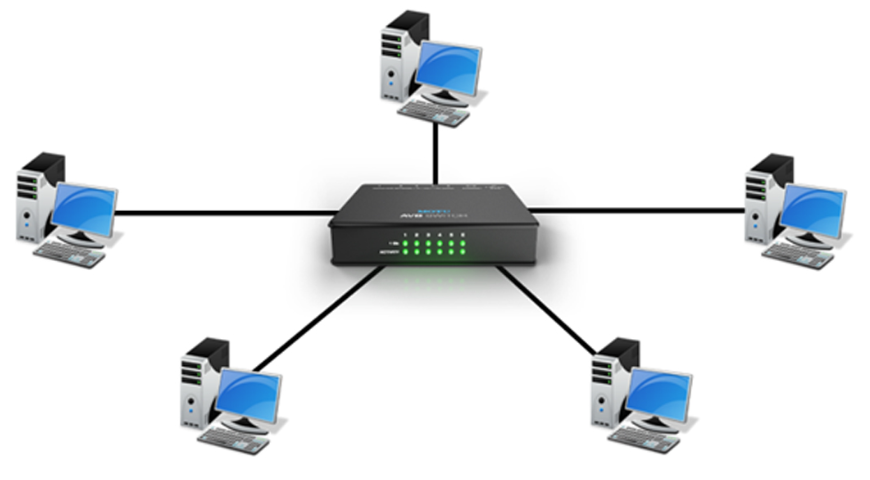
\includegraphics[width=0.5\textwidth]{img/hub.png}
	\caption{This is a sample image.}
\end{figure}

All theories, concepts, descriptions, ideas, and background information included in this section must be properly cited and referenced. The citation style used throughout the paper will be IEEE\footnote{IEEE uses a numerical citation system. The sources are indicated by a number in square brackets within the text, which corresponds to the full reference that must be included in the final bibliography. For more information on this system, consult \url{https://journals.ieeeauthorcenter.ieee.org/wp-content/uploads/sites/7/IEEE_Reference_Guide.pdf}}.

\subsection{Fundamental Concepts}
This section may include all concepts, definitions, and descriptions necessary to delve into the researched topic and help understand the problem being addressed.

\subsection{Background}
Previous studies and experiences related to the researched topic and a summary of the most important findings that help visualize the current state of science in the area of the addressed problem. The theoretical exposition should flow from the oldest to the most recent and from the broadest to the specific subject of the work.

At least five background studies will be required. The incorporated background must help to understand the current state of the topic and also provide a general overview of the solutions proposed by other authors to problems directly or indirectly related to the problem addressed in this work.

A proper literature review (focused on the problem statement and hypothesis, with current and relevant references) is a good indicator that, as a researcher, you have mastered the existing state of knowledge on your topic. The literature review is not a list of references, nor summaries of them, nor a compilation of vaguely related sources. Instead, it represents an integration of selectively chosen references that fulfill the outlined functions. In a few pages, you should discuss what studies have been previously conducted on the problem you will investigate and their main findings. When writing this section, you need to be very direct and concise, avoiding long definitions of concepts. We stress this: only include previous research that has specifically addressed your problem of interest. For instance, Trupke and Strassnig\cite{trupke2017} suggest including around 10 significant references. Including too many primary sources (especially when not directly linked to the topic) can bore the reader and leave out important references, which also suggests a lack of knowledge about a problem or phenomenon.

Finally, the links between questions and objectives, the theory, and the selected methods must be clear. Although this section does not present the entire methodology, you should include one or two paragraphs that connect theory with method at the end of the background section. This also helps to bridge this section with the next.

Some examples of initial wording for background paragraphs are shown in the following box:

\vspace{0.5cm}

\begin{table}[h]
	\begin{tabular}{| m{12cm} |}
		\hline
		\vspace{0.5cm}
		“In the literature relevant (linked, related, prior...) to our problem statement, it has been found that... (references) and... (reference)”

		\vspace{0.5cm}

		“Previous studies (references) have concluded that…”

		\vspace{0.5cm}

		“The background shows us that... (references)”

		\vspace{0.5cm}

		“Research has made it clear that... (references)...”

		\vspace{0.5cm}

		“On the other hand, it has also been discovered (demonstrated, highlighted, indicated... (references)...)”

		\vspace{0.5cm}

		“Furthermore, it has been concluded that... (references)”

		\vspace{0.5cm}

		\\
		\hline
	\end{tabular}
\end{table}

Also here is a example of a code, this can be changed and can be updated:
\noindent\textbf{Code example}
\begin{lstlisting}
// 1 Hz square wave on RC2
void init_compare(void){
    TRISC2_bit = 0;
    CCP1CON = 0b00000010;     // Compare, toggle output
    CCPTMRS0.C1TSEL = 0;      // Timer1
    CCPR1H = 0xF4;            
    CCPR1L = 0x24;
    T1CON = 0b00110001;       // Timer1 at 1 MHz tick
}
\end{lstlisting}
	
	% Section 3: Materials and Methods
	\section{Materials and Methods}

For the drafting of this section, it is recommended that students seek guidance from the course coordinator of the corresponding subject and their respective academic advisors.

\subsection{Work Approach}

This section describes the approach to be adopted for the project (quantitative, qualitative, mixed, technological project, or other) and details how the research will be conducted.

If the project is based on primary research (quantitative or qualitative studies), details must be provided regarding the research design according to its nature (experimental, non-experimental, etc.).

Additionally, a step-by-step explanation of all the research processes to be conducted is required. If the study involves a population and sample, these should be described. It is also necessary to detail the instruments and materials that will be used for data collection, as well as the tools to be employed in each process, in order to provide sufficient information to make the research replicable.

The processes described in this section are expected to be closely aligned with the achievement of the stated objectives.

\subsection{Technological Research}

If the project is based on technological research, the software development methodology to be used must be described, along with the activities to be carried out in the design, coding, integration, testing, and implementation phases.

To confirm the subsections and content to be included in this section, it is necessary to consult with the course coordinator and the respective project advisors.

	
	% Section 4: Data Analysis
	\section{Data Analysis}

(HOW THE ANALYSIS WILL BE CARRIED OUT AND WHAT BASIC TESTS WILL BE USED) AND PRELIMINARY RESULTS OR PILOT TESTS (IF AVAILABLE)

This section describes whether a pilot test is planned, how data collectors will be trained and how the data will be coded. Additionally, it should include an explanation of how access to the relevant information will be ensured.

If the project involves experimental designs, the procedures must clearly explain the nature of the treatment(s), the levels of the independent variable, the number of groups involved, the method for assigning participants or cases to groups, your role as a researcher in the experiment, the time span between pre-test, treatment, and post-test for each group, the way in which the groups will be monitored, and the location where the study will be conducted.

Regarding data analysis, Mertens\cite{mertens2015} includes the following:

\begin{itemize}
	\item \textit{Plan for processing the data:} coding, analytical software, and statistical tests to be used (for each hypothesis or variable; if no hypotheses were stated, then for each research question and variable).
	\item The way you will link the analysis or analyses to the research problem and hypotheses (it is not enough to mention which tests will be applied; you must establish the connection and the type of results expected).
\end{itemize}

Dahlberg, Wittink, and Gallo\cite{dahlberg2010} recommend adding, at the end of the methods section, a paragraph that explains the strengths and challenges of your research. This should include a description of alternative methods that could be considered and explain why the chosen method represents the best approach to the research problem. Alternatively, it should address how potential threats to the project and its feasibility will be managed. This paragraph demonstrates to reviewers and readers that you have anticipated problems, obstacles, and criticisms.

Additionally, you must honestly acknowledge the limitations of the study—something highly valued by all researchers.

	
	% Section 5: Anticipated Aspects
	\section{Anticipated Aspects}
ETHICAL ISSUES THAT CAN BE ANTICIPATED

You must clearly state your attitude of respect for the ethical aspects involved in the study (for example, confidentiality, anonymity, etc.). In some cases, authorization from an ethics committee and the consent of a specific group or institution will be required.


	
	% Section 6: Timeline
	\section{Timeline}

ETHICAL ISSUES THAT CAN BE ANTICIPATED

TIME SCHEDULE (SCHEDULING),

RESOURCES, MATERIALS, AND BUDGET

This section should contain a time table, schedule, or detailed programming of the actions you plan to carry out. The actions are listed on one side, and the time periods on the other. It is recommended that, when outlining tasks, you strike a balance between the general and the overly specific.
Time periods can be days, weeks, or months. The important thing about a time table is knowing when each stage begins and ends. It should also be realistic.

\subsection{Activity Schedule}
An example of the activity schedule is shown.

\subsection{Example 1 of an Activity Schedule}

\begin{table}[ht]
	\centering
	\renewcommand{\arraystretch}{1.5}
	\begin{tabular}{|c|m{6cm}|*{12}{c|}}
		\hline
		\multicolumn{2}{|c|}
        {\textbf{Schedule of activities}} & \multicolumn{12}{c|}{\textbf{DURATION MONTHS*}} \\
		\cline{3-14}
		\multicolumn{2}{|c|}{} & \multicolumn{1}{c|}{1} & \multicolumn{1}{c|}{2} & \multicolumn{1}{c|}{3} & \multicolumn{1}{c|}{4} & \multicolumn{1}{c|}{5} & \multicolumn{1}{c|}{6} & \multicolumn{1}{c|}{7} & \multicolumn{1}{c|}{8} & \multicolumn{1}{c|}{9} & \multicolumn{1}{c|}{10} & \multicolumn{1}{c|}{11} & \multicolumn{1}{c|}{12} \\
		\hline
		\textbf{N°} & \textbf{ACTIVITIES} & & & & & & & & & & & & \\
		\hline
		1 & Activity  1 & \checkmark  & & & & & & & & & & & \\
		\hline
		2 &  Activity  2 & & & & & & & & &  \checkmark & & & \\
		\hline
		& & & & & & & & & & & & & \\
		\hline
		& & & & & & & & & & & & & \\
		\hline
		& & & & & & & & & & & & & \\
		\hline
		& & & & & & & & & & & & & \\ 
		\hline
	\end{tabular}
	\caption{Description of the table.}
	\label{tab:cronograma}
\end{table}

\newpage


%Activity calendar template
\begin{landscape}

	\begin{table}[ht]
		\centering
		\begin{tabular}{c}
			\begin{ganttchart}[
				vgrid={draw=none, dotted},
				hgrid={draw=none},
				x unit=0.5cm,
				y unit title=0.6cm,
				y unit chart=0.6cm,
				title/.append style={draw=none, fill=none},
				title label font=\bfseries\footnotesize,
				title height=0.5,
				bar/.append style={fill=cyan},
				bar height=0.6
				]{1}{40}
				% Months
				\gantttitle{January}{4}
				\gantttitle{February}{4}
				\gantttitle{March}{4}
				\gantttitle{April}{4}
				\gantttitle{May}{4}
				\gantttitle{June}{4}
				\gantttitle{July}{4}
				\gantttitle{August}{4}
				\gantttitle{September}{4}
				\gantttitle{October}{4} \\
				% Weeks
				\gantttitle{Weeks}{40} \\
				\gantttitlelist{1,...,40}{1} \\
				
				\ganttbar{Review of instruments}{1}{4} \\
				\ganttbar{Pilot study}{5}{8} \\
				\ganttbar{Pilot analysis}{9}{12} \\
				\ganttbar{Redesign}{12}{15} \\
				\ganttbar{Sampling}{14}{17} \\
				\ganttbar{Fieldwork}{18}{20} \\
				\ganttbar{Data processing}{21}{24} \\
				\ganttbar{Analysis}{25}{28} \\
				\ganttbar{Final report}{29}{31}
			\end{ganttchart}
		\end{tabular}
		\caption{Schedule of Activities}
		\label{tab:gantt}
	\end{table}
\end{landscape}


\newpage



\subsection{Budget}

In the budget section, you may first present the total amount and then break down the most important categories, adding a more detailed breakdown in an appendix. Alternatively, you may begin with the itemized breakdown and conclude with the total. Resources may be expressed in monetary units (such as guaraníes, dollars, etc.), in kind (computers, analysis software, office space, among others), or in the form of concrete support (student assistants, permits, etc.).

According to The National Science Foundation\cite{NSF2014}, some common categories that may be included in the budget are:

\begin{itemize}
	\item \textbf{Direct costs} (those directly related to the project itself, such as salaries, permanent equipment, travel expenses, equipment maintenance, subcontracted services, publication charges, etc.).
	\item \textbf{Indirect costs} (those not directly impacting the project, such as accounting, building maintenance, project administration, etc.).
\end{itemize}


\subsection{Required Personnel}

\begin{table}[h]
	\centering
	\scriptsize % Reduce font size
	\renewcommand{\arraystretch}{1.5}
	\setlength{\tabcolsep}{5pt}
	\begin{tabular}{|c|m{3cm}|m{2cm}|m{2cm}|m{1.5cm}|m{1.5cm}|m{1.5cm}|m{1.5cm}|}
		\hline
		\textbf{No.} & \textbf{Full Name} & \textbf{Basic Profession} & \textbf{Postgraduate Degree} & \textbf{Main Role in the Project} & \textbf{Hours/Week} & \textbf{Duration (months)} & \textbf{Cost (thousands \$)} \\
		\hline
		1 &  & & & & & & \\
		\hline
		2 & & & & & & & \\
		\hline
		3 & & & & & & & \\
		\hline
		4 & & & & & & & \\
		\hline
		5 & & & & & & & \\
		\hline
		6 & & & & & & & \\
		\hline
		7 & & & & & & & \\
		\hline
	\end{tabular}
	\caption{Required Personnel}
\end{table}

\newpage
\subsubsection{Budget Table}
\begin{table}[h!]
	\centering
	\renewcommand{\arraystretch}{1.5}
	\setlength{\tabcolsep}{5pt}
	\begin{tabular}{|>{\raggedright\arraybackslash}m{11cm}|>{\raggedleft\arraybackslash}m{3cm}|}
		\hline
		\multicolumn{2}{|c|}{\textbf{BUDGET}} \\
		\hline
		\multicolumn{1}{|c|}{\textbf{Items and Lines}} & \multicolumn{1}{c|}{\textbf{Total}} \\
		\hline
		\textbf{Research Personnel} & \\ \hline
		1 principal investigator, salary \$1,600,000, half-time dedication, six months duration. & \$9,600,000 \\ 
		Indirect costs (multiplier 2.5) & \$12,000,000 \\ \hline
		2 co-investigators, salary \$1,200,000 each, 1/3 time dedication, 3 months duration each. & \$2,400,000 \\ 
		Indirect costs (multiplier 2.5) & \$6,000,000 \\ \hline
		1 research assistant (laboratory technician), salary \$500,000, full-time, 4 months duration. & \$2,000,000 \\ 
		Indirect costs (multiplier 2.5) & \$5,000,000 \\ \hline
		\textbf{Consumable Materials} & \\ \hline
		40 white rats (quotation 001 attached) & \$600,000 \\ 
		200 kg animal feed (quotation 3521) & \$800,000 \\ 
		25 boxes of hormone X (quotation 1328) & \$367,000 \\ 
		100 disposable syringes (quotation 1328) & \$20,000 \\ \hline
		\textbf{Equipment} & \\ \hline
		8 multiple cages (quotation 3511) & \$400,000 \\ 
		1 precision electronic scale, brand X (quotation A34281), donation requested. & \$1,200,000 \\ \hline
		\textbf{Miscellaneous Expenses} & \\ \hline
		Payment for data tabulation. Approximately 1,300 records at \$80 each (quotation 3821) & \$104,000 \\ 
		Half an hour of CPU time (quotation 3821) & \$300,000 \\ 
		Xerographic reproduction of reports, 20 copies, 100 pages at \$30 per page. & \$60,000 \\ \hline
		\textbf{Total} & \$40,851,000 \\ 
		\hline
	\end{tabular}
	
	\caption{Budget Table}
\end{table}



	
	% References
	\bibliographystyle{IEEEtran}
	\bibliography{bibliography/references}
	
	% Section 8: Appendices
	\addcontentsline{toc}{section}{Appendices} % Add Appendices to TOC
	\section*{Appendices}

Attachments are used to describe or illustrate in greater depth certain materials from the work that are not so important as to distract from the reading of the main text. They are also used to prevent the formatting of the document from being broken.
Examples: questionnaires used, source codes, additional statistical analysis, development of complicated formulas, photographs, etc. They should be titled and numbered and can be cited in the body of the document.

They may include maps of the site where a survey will be conducted, a measurement instrument already validated for the environment in which it will be applied, a photograph of the site where the experiment will be conducted, a figure showing the measurement equipment, etc. These elements are added only if they are required or you anticipate that their presentation will have a favorable effect.
	
\end{document}
